
\section{Węzły i~sploty}
Największą różnicą między węzłami matematycznymi oraz tymi z~prawdziwego jest życia jest to, że te pierwsze nie mają luźnych końców.
Można przyjąć nieidealną, naiwną definicję:

\begin{definition}[węzeł]
    Ciągłe oraz różnowartościowe odwzorowanie $S^1 \to \R^3$ nazywamy węzłem.
\end{definition}

\subsubsection{Rozróżnianie mutantów}
Żaden wielomianowy niezmiennik opisany w~tej książce nie potrafi odróżnić od siebie węzłów $11n_{34}$ oraz $11n_{42}$.
Okazuje się, że niewielomianowe niezmienniki też często są bezradne.

Niestety, dopuszcza ona patologiczne z~kombinatorycznego punktu widzenia węzły dzikie, jak ten z~rysunku \ref{fig:wild_knot}:

\begin{comment}
\begin{figure}
    \centering
    \label{fig:wild_knot}
    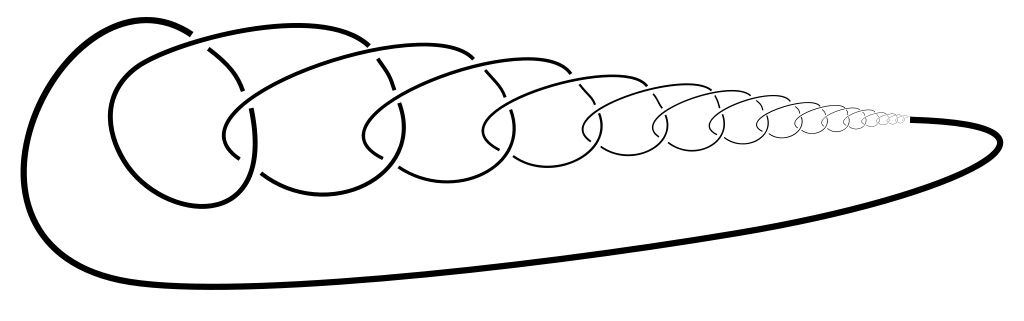
\includegraphics[width=0.5\linewidth]{wild_knot.png}
    \caption{Węzeł dziki}
\end{figure}
\end{comment}

Zastanówmy się, jakim formalizmem opisać manipulowanie fizycznym sznurkiem, by wykluczyć węzły dzikie z~naszych rozważań.
Nie można użyć izotopii (dwa węzły są izotopijne, jeśli istnieje ciągła funkcja $F \colon S^1 \times [0, 1] \to \R^3$ taka, że $F(-, 0)$ jest pierwszym, zaś $F(-,1)$ drugim węzłem), gdyż każdy węzeł jest izotopijny z punktem:

% TODO: Tu brakuje obrazka.

W podobny sposób moglibyśmy przekształcić dowolny węzeł w~niewęzeł.
Teoria, w~której wszystkie obiekty są takie same, nie jest zbyt ciekawa.
Zwykła izotopia nie oddaje dobrze tego, czym jest równoważność węzłów wykonanych z~prawdziwego sznurka.
Trzeba od niej wymagać dodatkowo, by była gładka albo lokalnie płaska.
Z twierdzenia o rozszerzaniu izotopii wynika, że można ją wtedy podnieść do izotopii otaczającej.
Ta ostatnia uwzględnia, jak węzeł leży w~przestrzeni i okazuje się być właściwym pojęciem równości dla teorii węzłów:

% DICTIONARY;isotopy;izotopia;-
% DICTIONARY;ambient;otaczająca;izotopia
\begin{definition}[izotopia otaczająca]
    Niech $N, M$ będą rozmaitościami, zaś $K_1, K_2 \colon N \to M$ włożeniami.
    Ciągłe odwzorowanie $F \colon M \times [0,1] \to M$ spełniające następujące warunki:
    \begin{enumerate}
        \item funkcja $F(-, 0)$ jest odwzorowaniem tożsamościowym,
        \item każda z funkcji $F(-, t)$ jest homeomorfizmem,
        \item złożenie $F(-, 1)$ z pierwszym włożeniem $K_1$ daje drugie włożenie $K_2$
    \end{enumerate}
    nazywamy izotopią otaczającą przenoszącą $K_1$ na $K_2$.
\end{definition}

W topologii rozważa się włożenia dowolnych rozmaitości, nam wystarczy jeden szczególny przypadek $N = S^1$ oraz $M = \R^3$.
Intuicyjnie, funkcja $F$ zniekształca przestrzeń $\R^3$ tak, że w~chwili początkowej $t = 0$ widzimy pierwszy, zaś w~chwili końcowej $t = 1$ drugi węzeł.
Izotopia otaczająca nie pozwala na ściąganie zaplątanych fragmentów do punktu.

% TODO: Homeomorfizmy $F_t$ można zastąpić przez dyfeomorfizmy zachowujące orientację.

% DICTIONARY;knot;węzeł;-
% DICTIONARY;tame;poskromiony;węzeł
% DICTIONARY;wild;dziki;węzeł
\begin{definition}[węzeł]
    \label{def:knot}
    \index{węzeł}
    Gładkie włożenie $S^1 \to \R^3$ otaczająco izotopijne z~zamkniętą łamaną bez samoprzecięć nazywamy węzłem poskromionym.
    Dwa węzły są równoważne, jeśli istnieje pomiędzy nimi izotopia otaczająca.
\end{definition}

Przez prawie całą książkę interesować nas będą jedynie węzły poskromione, czyli takie które nie są dzikie,
dlatego jeśli nie zaznaczono inaczej, od teraz pisząc węzeł mamy na myśli węzeł poskromiony.
Istnieje jeszcze jedna, konkurencyjna definicja węzłów równoważnych:

\begin{proposition}
    \label{def:equivalent_knots_2}
    Dwa węzły są równoważne, gdy jeden z~nich jest obrazem drugiego przez zachowujący orientację homeomorfizm $\R^3 \to \R^3$.
\end{proposition}

Stwierdzenie to przestaje być prawdziwe po zastąpieniu przestrzeni $\R^m$ przez $S^m$.

\begin{proof}
    Podany niżej dowód pochodzi z~książki ,,Topology from the differentiable viewpoint'' Johna Milnora.
    Musimy pokazać, że dyfeomorfizm $f \colon \R^m \to \R^m$ jest gładko izotopijny z~identycznością.
    Translacje są izotopiami, więc bez straty ogólności zakładamy, że $f(0) = 0$.
    Pochodna $f$ w~zerze jest dana wzorem $\mathrm{d}f_0(x) = \lim_{t \to 0} f(tx) /t$,
    naturalną definicję izotopii $F \colon \R^m \times [0, 1] \to \R^m$ stanowi więc
    \[
        F(x, t) = \begin{cases}
            \mathrm{d}f_0(x) & t = 0 \\
            f(tx) / t & 0 < t \le 1
        \end{cases} .
    \]

    Funkcja $F$ jest gładka, gdyż na mocy lematu Hadamarda funkcja $f$ zapisuje się jako suma $x_1 g_1(x) + \ldots + x_mg_m(x)$, gdzie funkcje $g_i$ są gładkie, co jakoś kończy dowód.
\end{proof}

Formalnie węzły to pewne odwzorowania, więc prawidłowym sposobem na zapisanie, że są izotopijne (czyli dla nas: równe), jest $K_1 \simeq K_2$.
Ponieważ nie prowadzi to do problemów, będziemy jednak stosować zapis $K_1 = K_2$.
Jednocześnie często węzeł (jako odwzorowanie) nie będzie odróżniany od obrazu tego odwzorowania.

% DICTIONARY;link;splot;-
% DICTIONARY;component;ogniwo splotu;-
\begin{definition}[splot, ogniwo]
    \index{splot}
    Sumę parami rozłącznych węzłów $K_1, K_2, \ldots, K_n$ nazywamy splotem.
    Składniki sumy nazywamy ogniwami.
\end{definition}

Przez analogię do węzłów mówimy, że dwa sploty są takie same, jeśli jeden jest obrazem drugiego przez zachowujący orientację homeomorfizm $\R^3 \to \R^3$.
W~takiej sytuacji obydwa sploty mają tyle samo ogniw.

\begin{example}
    \index{splot!Hopfa}
    Splot Hopfa to najprostszy splot nietrywialny, którym w~1931 r. zajmował się Heinz Hopf, topolog niemiecki, w~ramach badań nad tzw. rozwłóknieniem (Hopf fibration).
\end{example}

\begin{example}
    \index{splot!Whiteheada}
    Whitehead w~1934 odkrył kontrprzykład do nieudanego dowodu hipotezy Poincarego.
    Był nim splot o~dwóch składowych przedstawiony na poniższym rysunku.
\end{example}

\begin{comment}
    \begin{figure}[H]
        \begin{minipage}[b]{.48\linewidth}
            \centering
            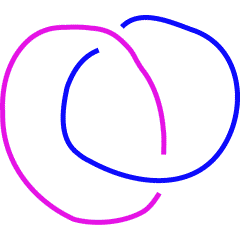
\includegraphics[width=0.5\linewidth]{../data/mixed/L2a1.png}
            \subcaption{splot Hopfa}
        \end{minipage}
        \begin{minipage}[b]{.48\linewidth}
            \centering
            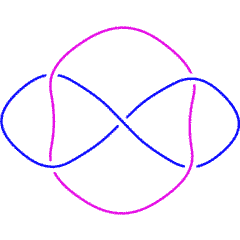
\includegraphics[width=0.5\linewidth]{../data/mixed/L5a1.png}
            \subcaption{splot Whiteheada}
        \end{minipage}
    \end{figure}
\end{comment}

Jeśli dwa węzły są równoważne, to ich dopełnienia są oczywiście homeomorficzne.
Pytanie o~prawdziwość implikacji odwrotnej jako pierwszy zadał najprawdopodobniej  Tietze \cite{tietze08} w~1908 roku.
W roku 1987 pokazano, że istnieją co najwyżej dwa węzły o~zadanym dopełnieniu (Culler, Gordon, Luecke, Shalen \cite{culler87}).
Dwa lata później poznaliśmy pozytywną odpowiedź na pytanie Tietzego: każdy węzeł jest wyznaczony jednoznacznie przez swoje dopełnienie.

\begin{theorem}[Gordon, Luecke, 1989]
    \label{thm:gordon_luecke}
    \index{twierdzenie!Gordona-Lueckego}
    Poskromione węzły o~homeomorficznych (z zachowaniem orientacji) dopełnieniach są wzajemnie izotopijne.
\end{theorem}

\begin{proof}[Niedowód]
\index{człowiek!Gordon, Cameron}%
\index{człowiek!Luecke, John}%
    Wynika to z~ogólniejszego stwierdzenia:
    nietrywialna chirurgia Dehna na węźle w~3-sferze nigdy nie daje 3-sfery.
    Pełny dowód zawiera praca \cite{gordon89}.
\end{proof}

Twierdzenie to zamienia problem lokalny (czy dwa węzły w kuli $S^3$ są równoważne?) w~problem globalny (czy dwie przestrzenie topologiczne są homeomorficzne?).
Whitehead w~pracy \cite{whitehead37} z~1937 roku podał nieskończenie wiele splotów, których dopełnienia wyglądają jak dopełnienia splotu Whiteheada.
\index{człowiek!Whitehead, John}%
Odpowiednik twierdzenia \ref{thm:gordon_luecke} dla splotów jest więc fałszywy.

% TODO: przesunąć to gdzieś dalej, za definicję skrzyżowania
Poniższa definicja nie jest nam jeszcze potrzebna, ale wygodnie przytoczyć ją już teraz.

% DICTIONARY;splittable;rozszczepialny;splot
\begin{definition}[rozszczepialność]
    \index{splot!rozszczepialny}
    Jeżeli splot $L$ można zanurzyć w przestrzeni $\R^3$ tak, że niektóre jego ogniwa będą leżeć nad pewną rozłączną ze splotem płaszczyzną, zaś pozostałe pod nią, to powiemy, że splot $L$ jest rozszczepialny.
\end{definition}

Liczbę nierozszczepialnych splotów, pierwszych lub złożonych, zebrano w tabeli.
Źródło: baza danych OEIS, ciąg \href{https://oeis.org/A086825}{A086825}.

\renewcommand*{\arraystretch}{1.4}
\footnotesize
\begin{longtable}{lccccccccc}
    \hline
    \textbf{skrzyżowania}  &  0  &  1  &  2  &  3  &  4  &  5  &  6   &  7   &  8   \\  \hline  \endhead
    sploty                 &  1  &  0  &  1  &  1  &  3  &  4  &  15  &  24  &  82  \\
    \hline
\end{longtable}
\normalsize

Teoria węzłów bada przede wszystkim węzły, ale istnieją jej odmiany skupiające się na innych, pokrewnych obiektach.
Mamy na przykład węzły obramowane:

% DICTIONARY;frame;obramowany;węzeł
% DICTIONARY;framing;obramowanie;-
\begin{definition}[obramowanie]
\index{obramowanie|see {węzeł obramowany}}%
\index{węzeł!obramowany}%
    Każde nieznikające normalne pole wektorowe na splocie nazywamy obramowaniem.
    Jeżeli wszystkie wektory są równoległe do płaszczyzny, na której leży diagram tego splotu, obramowanie nazywamy płaskim\footnote{Po angielsku ,,blackboard framing'', ale nie da się tego sensownie przetłumaczyć...}.
\end{definition}

% Liczba samozaczepienia zorientowanego obramowanego splotu $L$ to indeks zaczepienia tego splotu ze sobą pchniętym w kierunku obramowania, jej wartość to dokładnie spin.

% DICTIONARY;virtual;wirtualny;węzeł
% DICTIONARY;welded;zespawany;węzeł
% DICTIONARY;long;długi;węzeł
Są jeszcze węzły wirtualne, zespawane (iloraz węzłów wirtualnych przez ruch znany jako ,,nadskrzyżowania komutują''), długie (gdzie końce nie są ze sobą zszyte, ale umieszczone tak daleko, że są nieosiągalne) i inne.
Ta książka nie zawiera zbyt wiele informacji o wspomnianych bytach.
% http://katlas.org/ester/weldedknots/explanations.html
% koniec sekcji Węzły i sploty

